\section{Objectif}

\subsection{Archétype}
    L'objectif du projet est de réaliser un jeu s'inspirant du jeu de stratégie Risk, avec des règles simplifiées.
    
\subsection{Règles du jeu}
    Au début du jeu, le joueur reçoit des territoires puis gère ses armées en les plaçant sur les pays qu'il possède. A tour de rôle, les deux adversaires s'attaquent afin de gagner des territoires. Le vainqueur est celui qui conquiert les 2/3 des pays présents sur le plateau de jeu (nous pourrons modifier cet aspect du jeu pour que les parties durent moins longtemps). Pour cela, il doit lancer des dés qui décideront de l'issue du combat entre deux territoires. Le joueur peut perdre des armées à chaque phase de jeu et en reçoit de nouvelles à diverses occasions. Un joueur perd un territoire lorsqu'il n'a plus d'armée dessus. 
    \newline
    \newline
    Le joueur qui attaque peut décider d'attaquer avec 1, 2 ou 3 armées à condition d'avoir au moins ce nombre d'armées en poste sur le territoire. Le joueur qui défend peut défendre avec 1 ou 2 armées à condition d'avoir au moins ce nombre d'armées sur le territoire, le nombre d'armées sur un territoire n'étant pas limité.
    \begin{itemize}
        \item Si l'attaquant joue avec 1 armée, la défense peut défendre avec 1 ou 2 armées. Si le plus grand lancer de dé du défenseur est supérieur ou égal à celui de l'attaquant, c'est l'attaquant qui perd une armée. Sinon, le défenseur perd une armée. 
        \item L'attaquant peut jouer avec 2 armées. Si la défense joue avec 1 armée, la perte possible est de 1 de chaque côté. Si la défense joue avec 2 armées, la perte maximale est de 2 armées de chaque côté. 
        \item L'attaquant joue avec 3 armées. Le cas de figure est identique au précédent bien que l'attaque ait une proportion de victoire plus importante. Le défenseur ne peut pas mettre en jeu plus de 2 armées, et donc ne peut pas perdre plus de 2 armées lors d'une attaque. Vous trouverez un exemple sur la page suivante. 
        \newline
        \newline
    \end{itemize}

    Un joueur ne peut attaquer qu'un pays frontalier au sien. 
    \newline
    A la fin de son tour, un joueur peut effectuer des déplacements stratégiques. Il peut alors déplacer des armées d'un pays qu'il possède à un autre pays qu'il possède à condition que ces deux pays soient frontaliers.

\begin{figure}[!htbp]
        \centering
        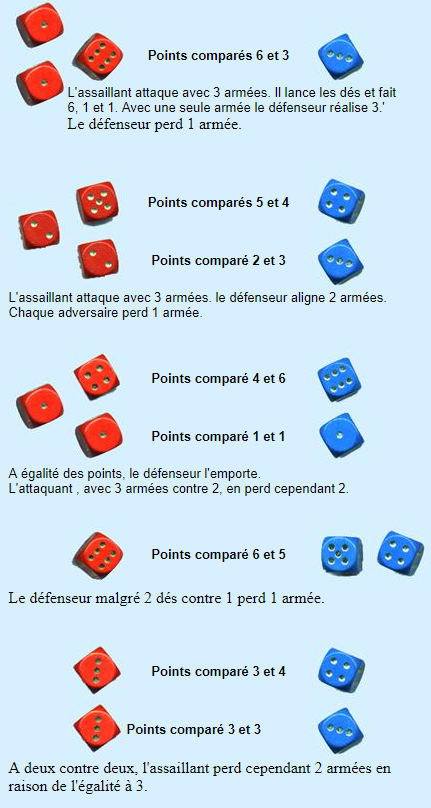
\includegraphics[width=11cm]{Images/des_riskk.PNG}
        \caption{Exemple de lancé de dés}
    \end{figure}
\newpage 

\subsection{Ressources}
    Plusieurs ressources sont nécessaires pour afficher l'état du jeu au cours de la partie. 
    Le joueur joue sur un plateau représentant le monde. Chaque continent est représenté par une couleur (figure \ref{fig:textures_plateau} et figure \ref{fig:textures_plateau2}). Les armées sont représentées par des pions (figure \ref{fig:textures_pions}). Le nombre d'armées par territoire sera indiqué par un nombre. Enfin, lorsqu'il conquiert un territoire, le joueur reçoit une carte qui pourra lui donner des avantages (figure \ref{fig:textures_cartes}). Les éléments ressources seront améliorés au fur et à mesure de la conception. 
    
    \begin{figure}[!htbp]
        \centering
        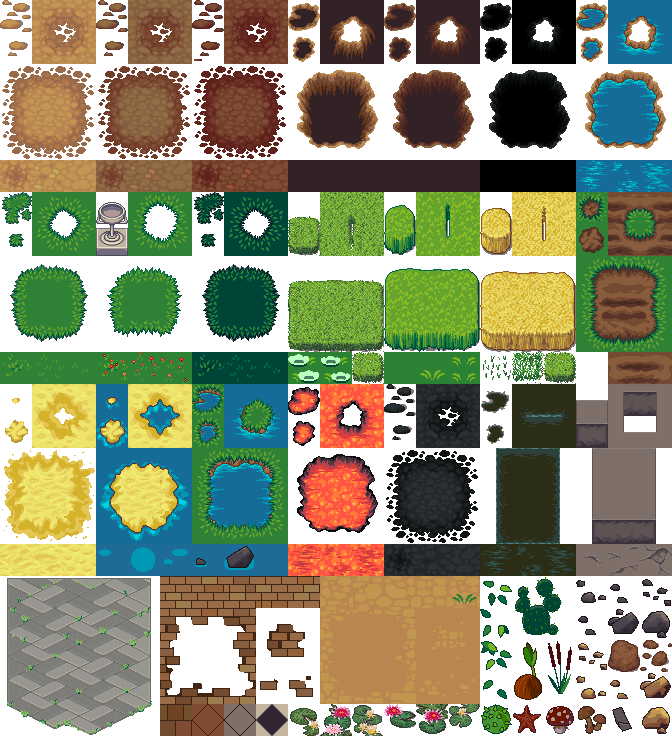
\includegraphics[width=6cm]{Images/terrain.png}
        \caption{Textures pour le plateau}
        \label{fig:textures_plateau}
    \end{figure}

    
    \begin{figure}[!htbp]
        \centering
        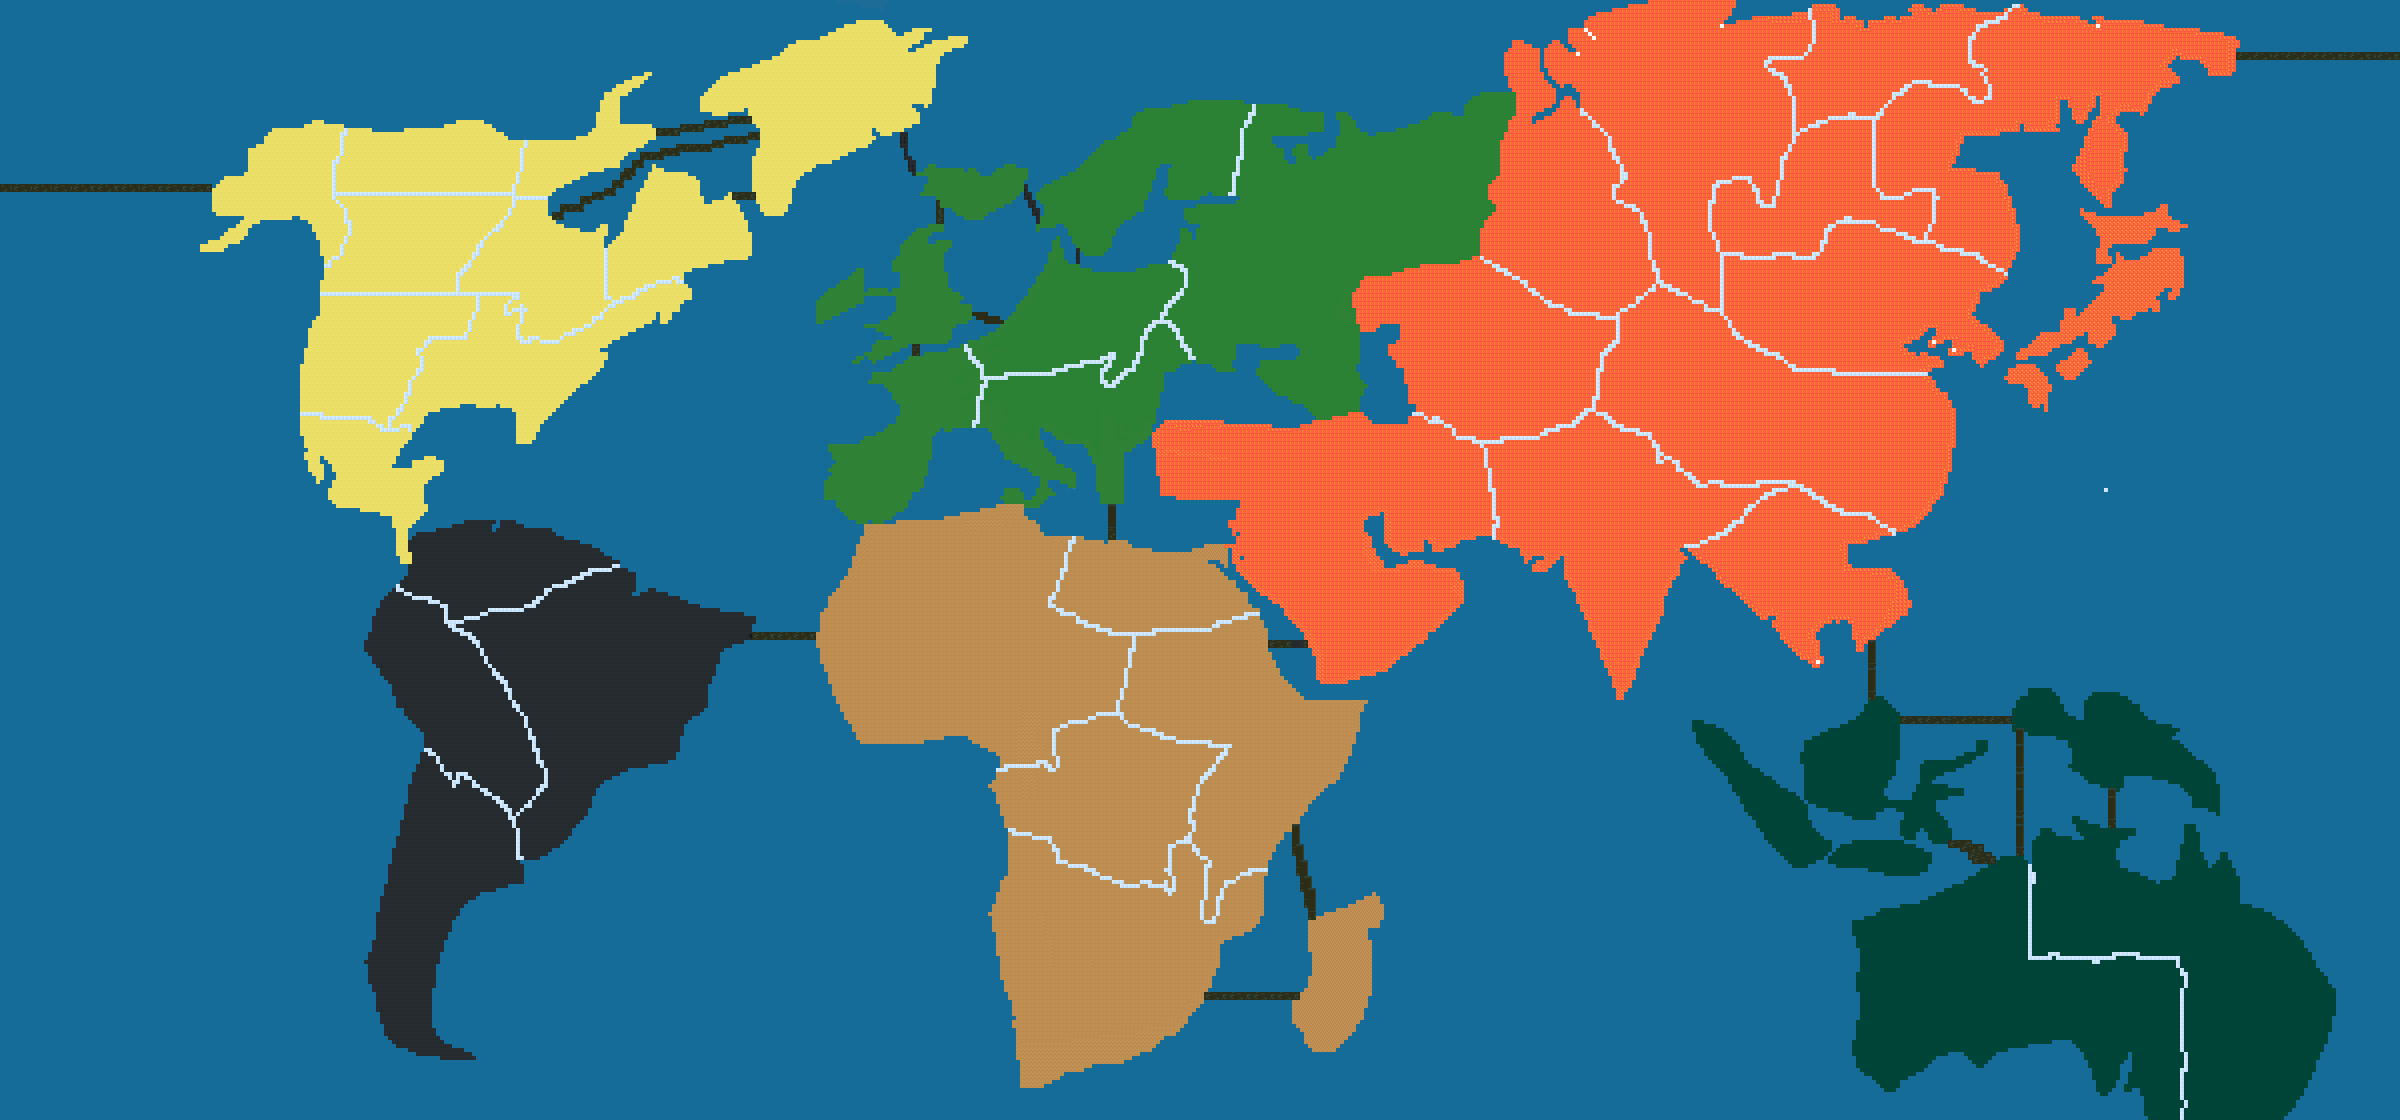
\includegraphics[width=13cm]{Images/map_jeu.png}
        \caption{Textures pour la plateau}
        \label{fig:textures_plateau2}
    \end{figure}
    
    \begin{figure}[!htbp]
        \centering
        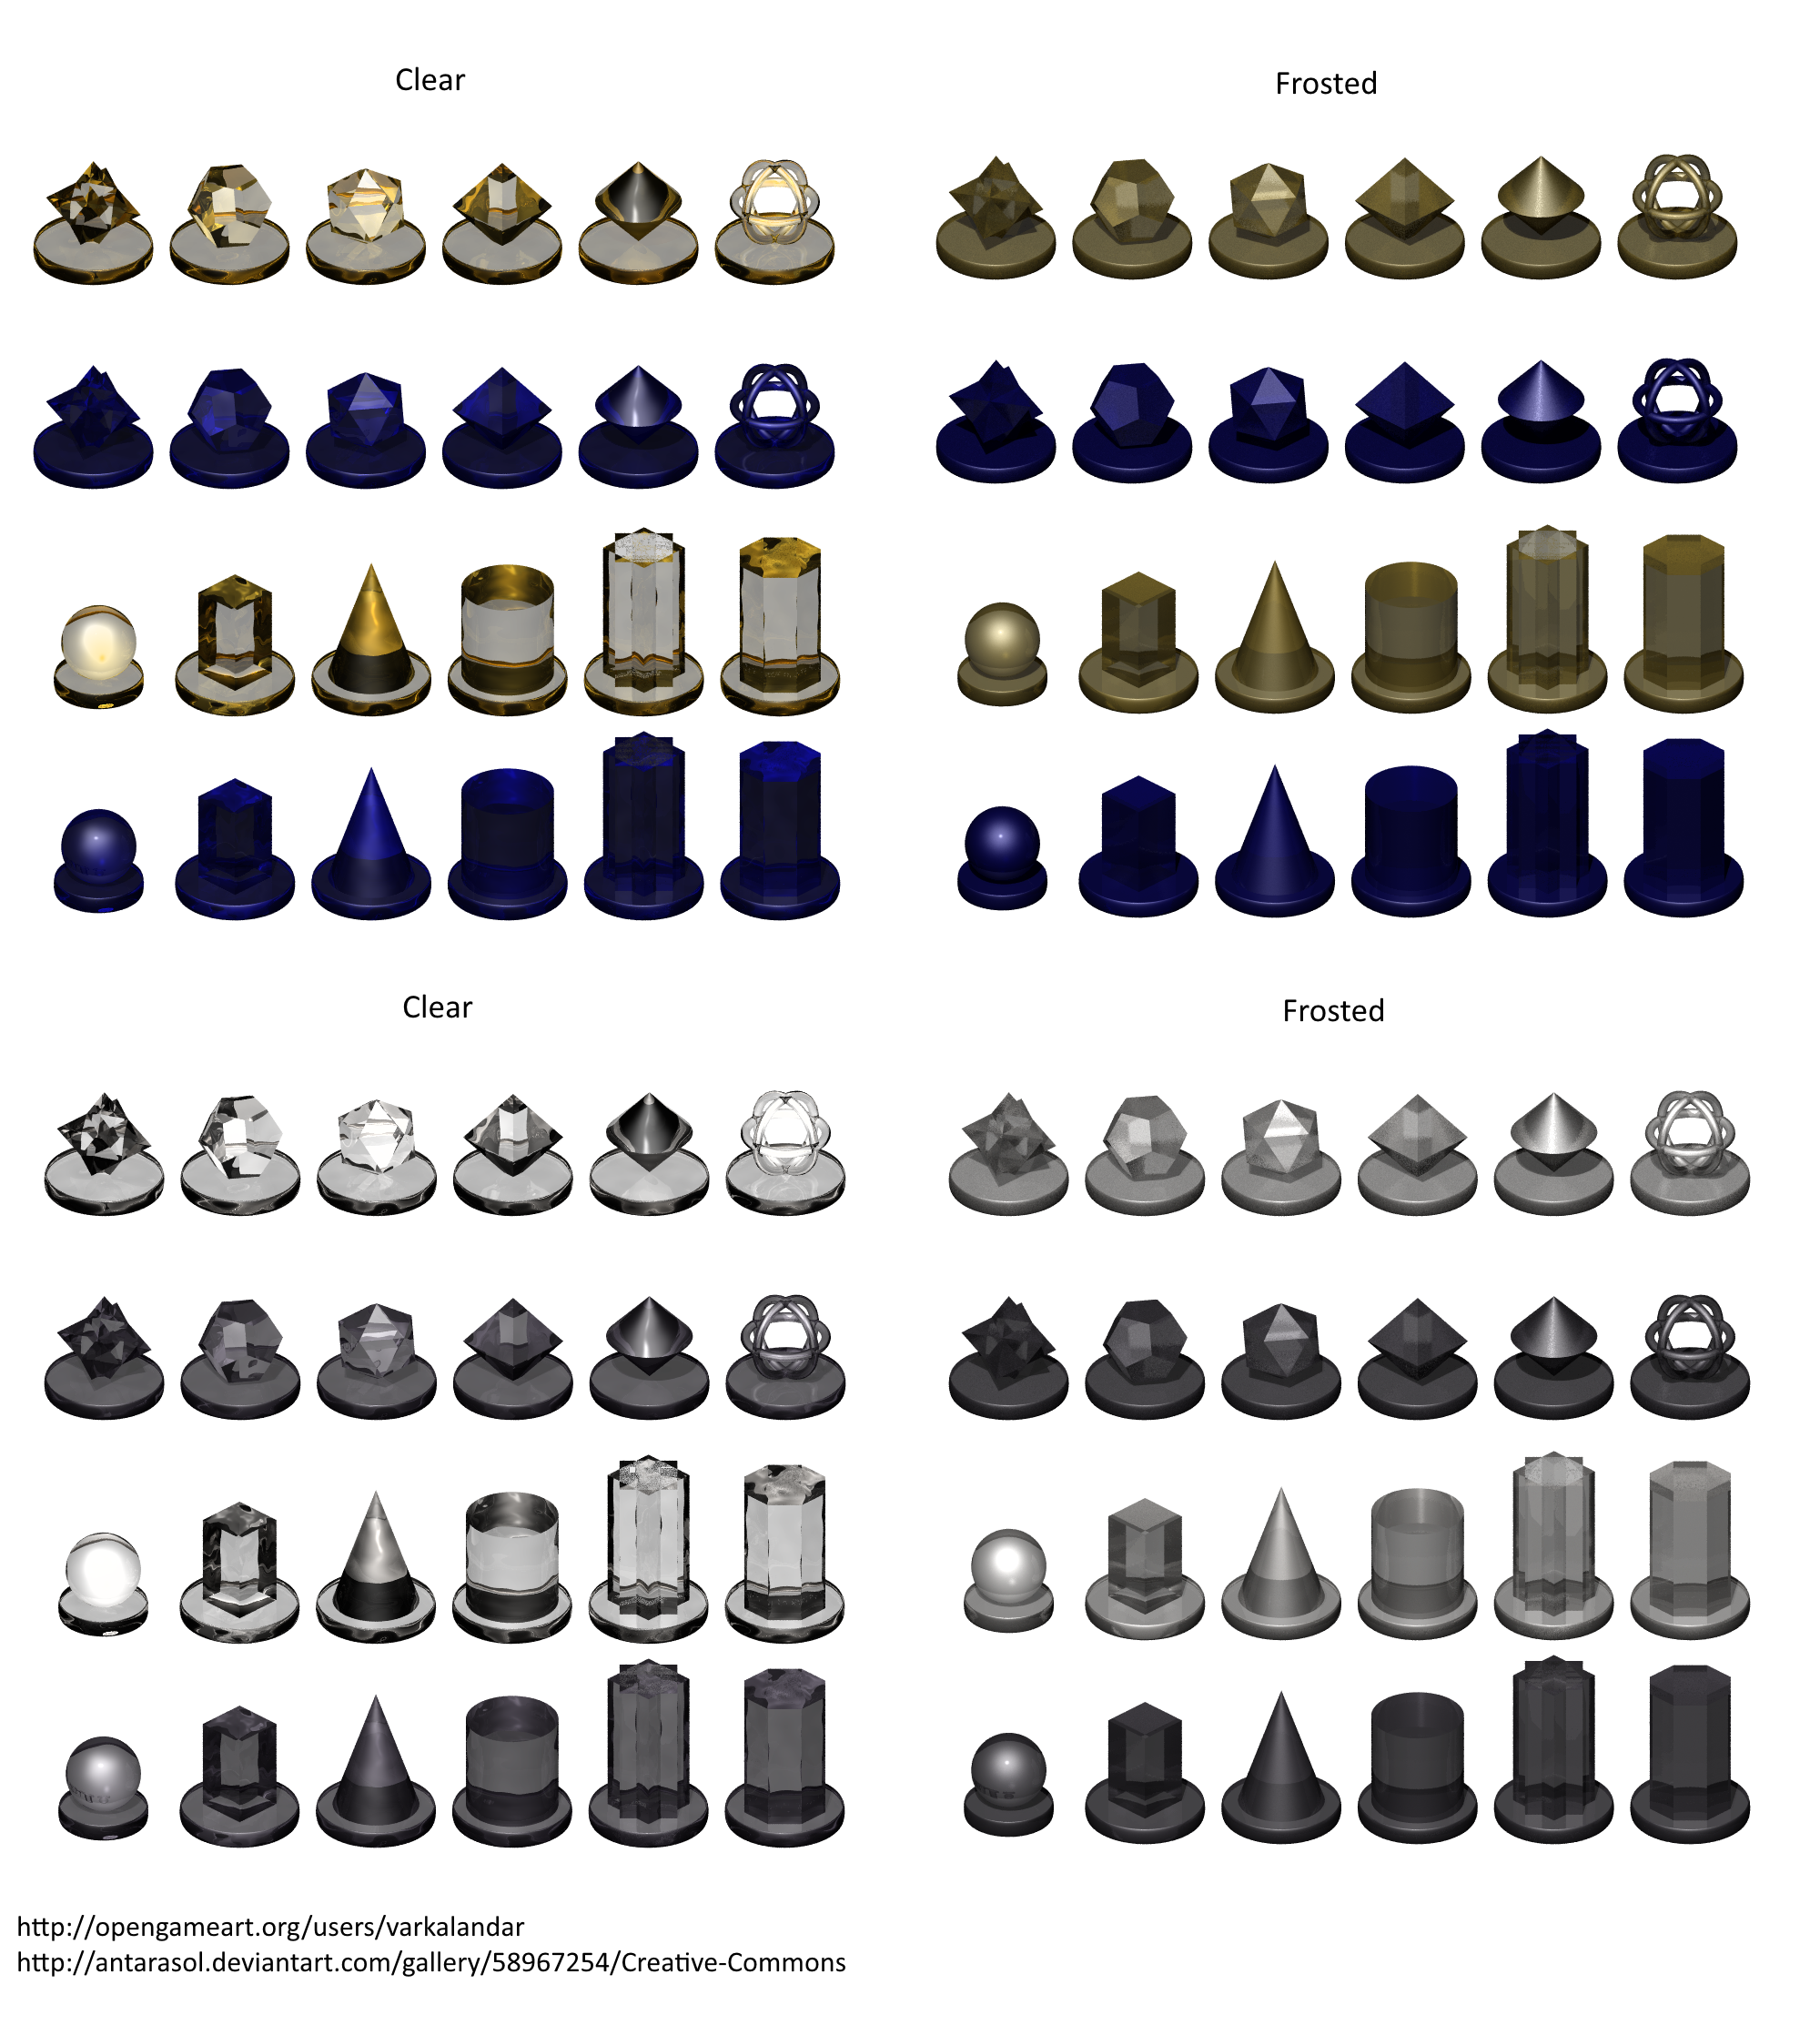
\includegraphics[width=6cm]{Images/pions.png}
        \caption{Textures pour les pions}
        \label{fig:textures_pions}
    \end{figure}
    
    \begin{figure}[!htbp]
        \centering
        
\includegraphics[width=14cm]{Images/cartes.png}
        \caption{Textures pour les cartes}
        \label{fig:textures_cartes}
    \end{figure}